Die allink GmbH wurde 2005 von den drei Partner David Zangger, Christoph Schlatter
und Michael Walder gegründet. David Zangger und Christoph Schlatter kümmern sich
seit jeher als Creative Directors um die grafischen Umsetzungen und die Designqualität.
Michael Walder kümmerte sich bis 2010 nebst den geschäftsführerischen Tätigkeiten
auch um die ganze Informatik. Nach der Fusionierung mit der SiSprocom übergab
er die Leitung der Informatik an Silvan Spross ab und widmet sich nun dem Aufbau der
Beratung und Projektleitung. Seit 2010 bezeichnet sich allink als die interdisziplinäre 
und marktnahe Designagentur, wie man ihrer Website entnehmen kann:

\begin{quote}
``allink.creative ist eine Designagentur, die Produkte, Marken und Unternehmen 
attraktiv und einzigartig in Szene setzt. Unser Design soll Menschen erreichen 
und begeistern. Weil wir marktnah arbeiten, stellen wir den wirtschaftlichen 
Nutzen von Design stets in den Vordergrund.
Wir arbeiten interdisziplinär, damit wir die breiten Möglichkeiten an 
Kommunikationskanälen optimal für unsere Kunden einsetzen können. Unser 
Team von Spezialisten aus den vielfältigsten Bereichen findet innovative 
und gesamtheitliche Lösungen, um Marken und Firmen wirkungsvoll zu positionieren. 
Die Bereiche Branding, Online Communication, Packaging Design und Product 
Design zählen dabei zu unseren Kernkompetenzen.''\footnote{Vgl. Rubrik ``About'' 
auf der Website von allink, \url{http://allink.ch/}}
\end{quote}

Das Unternehmen lässt sich zur Zeit in die drei Hauptbereiche Beratung, Grafik
und Informatik unterteilen. Diese Aufteilung ist in der Abbildung \ref{pic:04_funktionales_organigramm}
dargestellt.

\begin{figure}[htbp]
\begin{center}
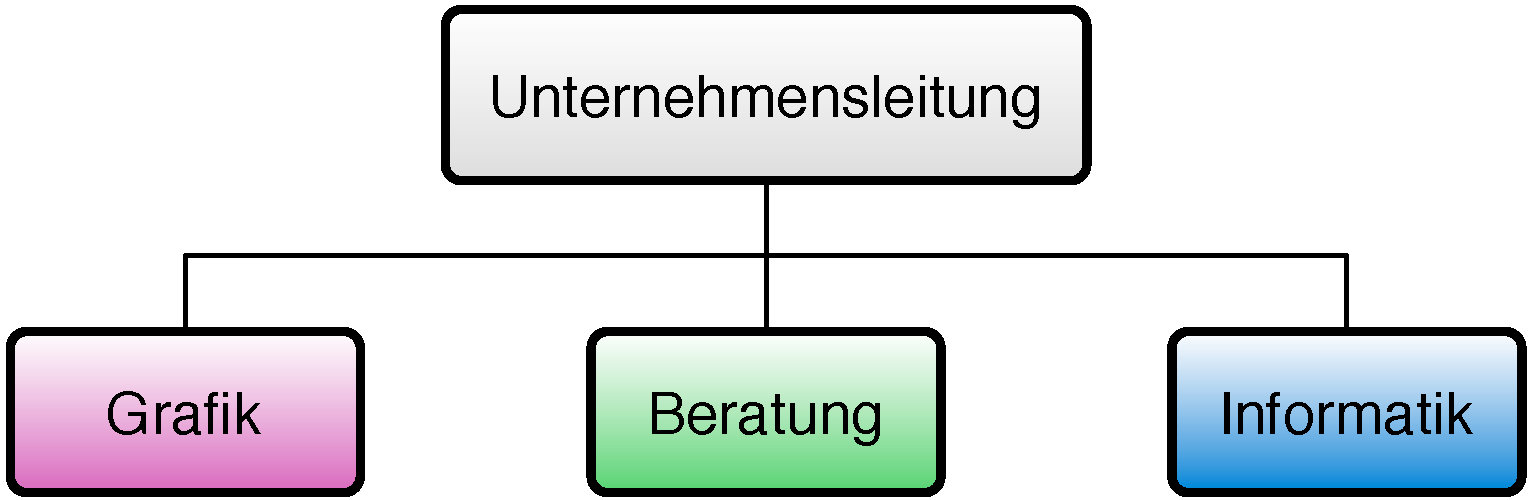
\includegraphics[width=0.46\textwidth,angle=0]{./bilder/analyse/04_funktionales_organigramm.pdf}
\caption[]{Funktionales Organigramm von allink\footnotemark}
\label{pic:04_funktionales_organigramm}
\end{center}
\end{figure}
\footnotetext{Eigene Darstellung}

Wobei sich jeweils ein bis zwei Partner um einen
Bereich kümmern. Dies beinhaltet nebst den Alltagsarbeiten auch organisatorische 
Aufgaben wie das Personalmanagement und die Verteilung der Arbeitspakete an den 
geeignetsten Mitarbeiter. In der Grafik \ref{pic:mitarbeiter_pro_bereich} 
sind die Mitarbeiter pro Bereich abgebildet.

\begin{figure}[htbp]
\begin{center}
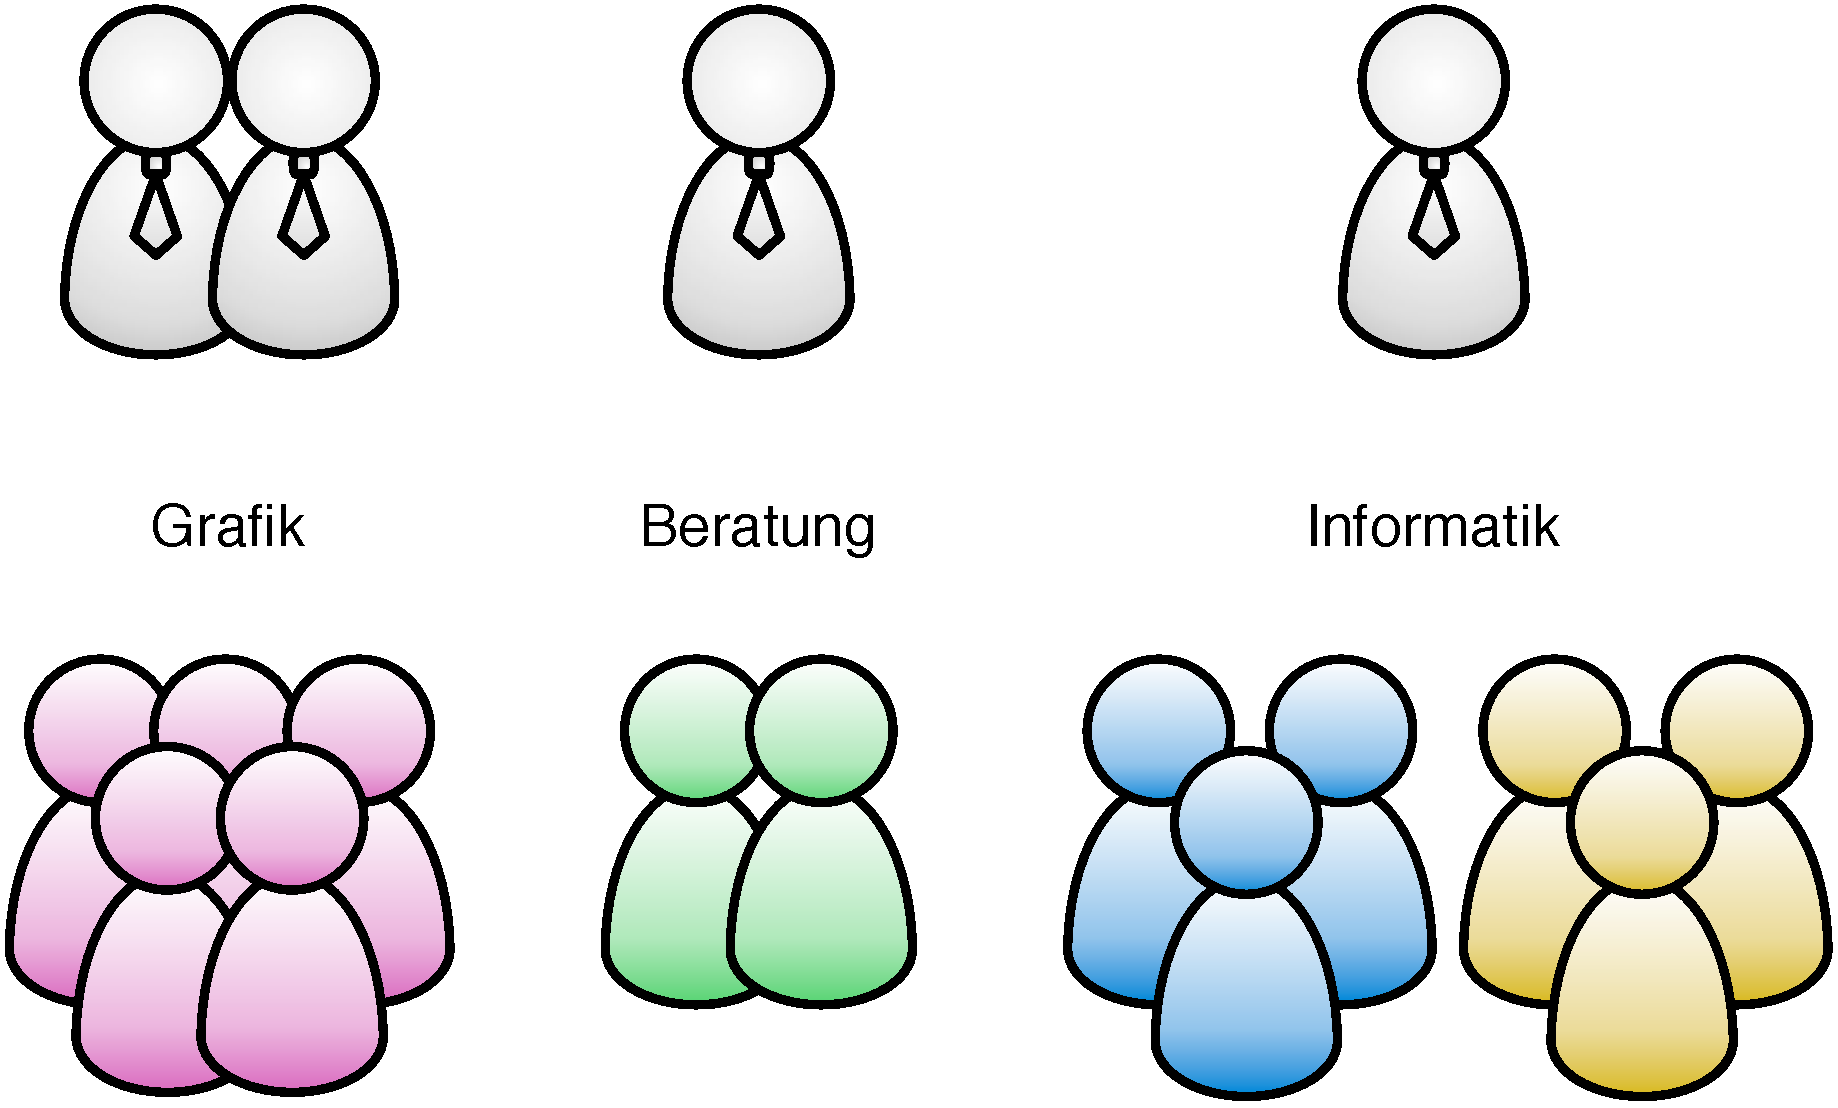
\includegraphics[width=0.55\textwidth,angle=0]{./bilder/analyse/mitarbeiter_pro_bereich.pdf}
\caption[]{Übersicht der Mitarbeitern pro Bereich\footnotemark}
\label{pic:mitarbeiter_pro_bereich}
\end{center}
\end{figure}
\footnotetext{Eigene Darstellung}

Im Bereich Grafik sind nebst drei Vollzeitangestellen noch ein Praktikant und eine
Lehrtochter angestellt. In der Beratung beschäftigt allink zur Zeit zwei Mitarbeiter.
Die Informatik setzt sich aus zwei Vollzeitangestellten sowie einem Pratikant
zusammen. Die drei weiteren Informatiker arbeiten als externe Berater und
werden höchst selten in einem internen Projekt beschäftigt.

Trotz dieser Aufteilung in mehrere Bereiche geht der Kommunikationsweg nicht
immer über die für den Mitarbeiter zuständigen Partner. 

\begin{figure}[htbp]
\begin{center}
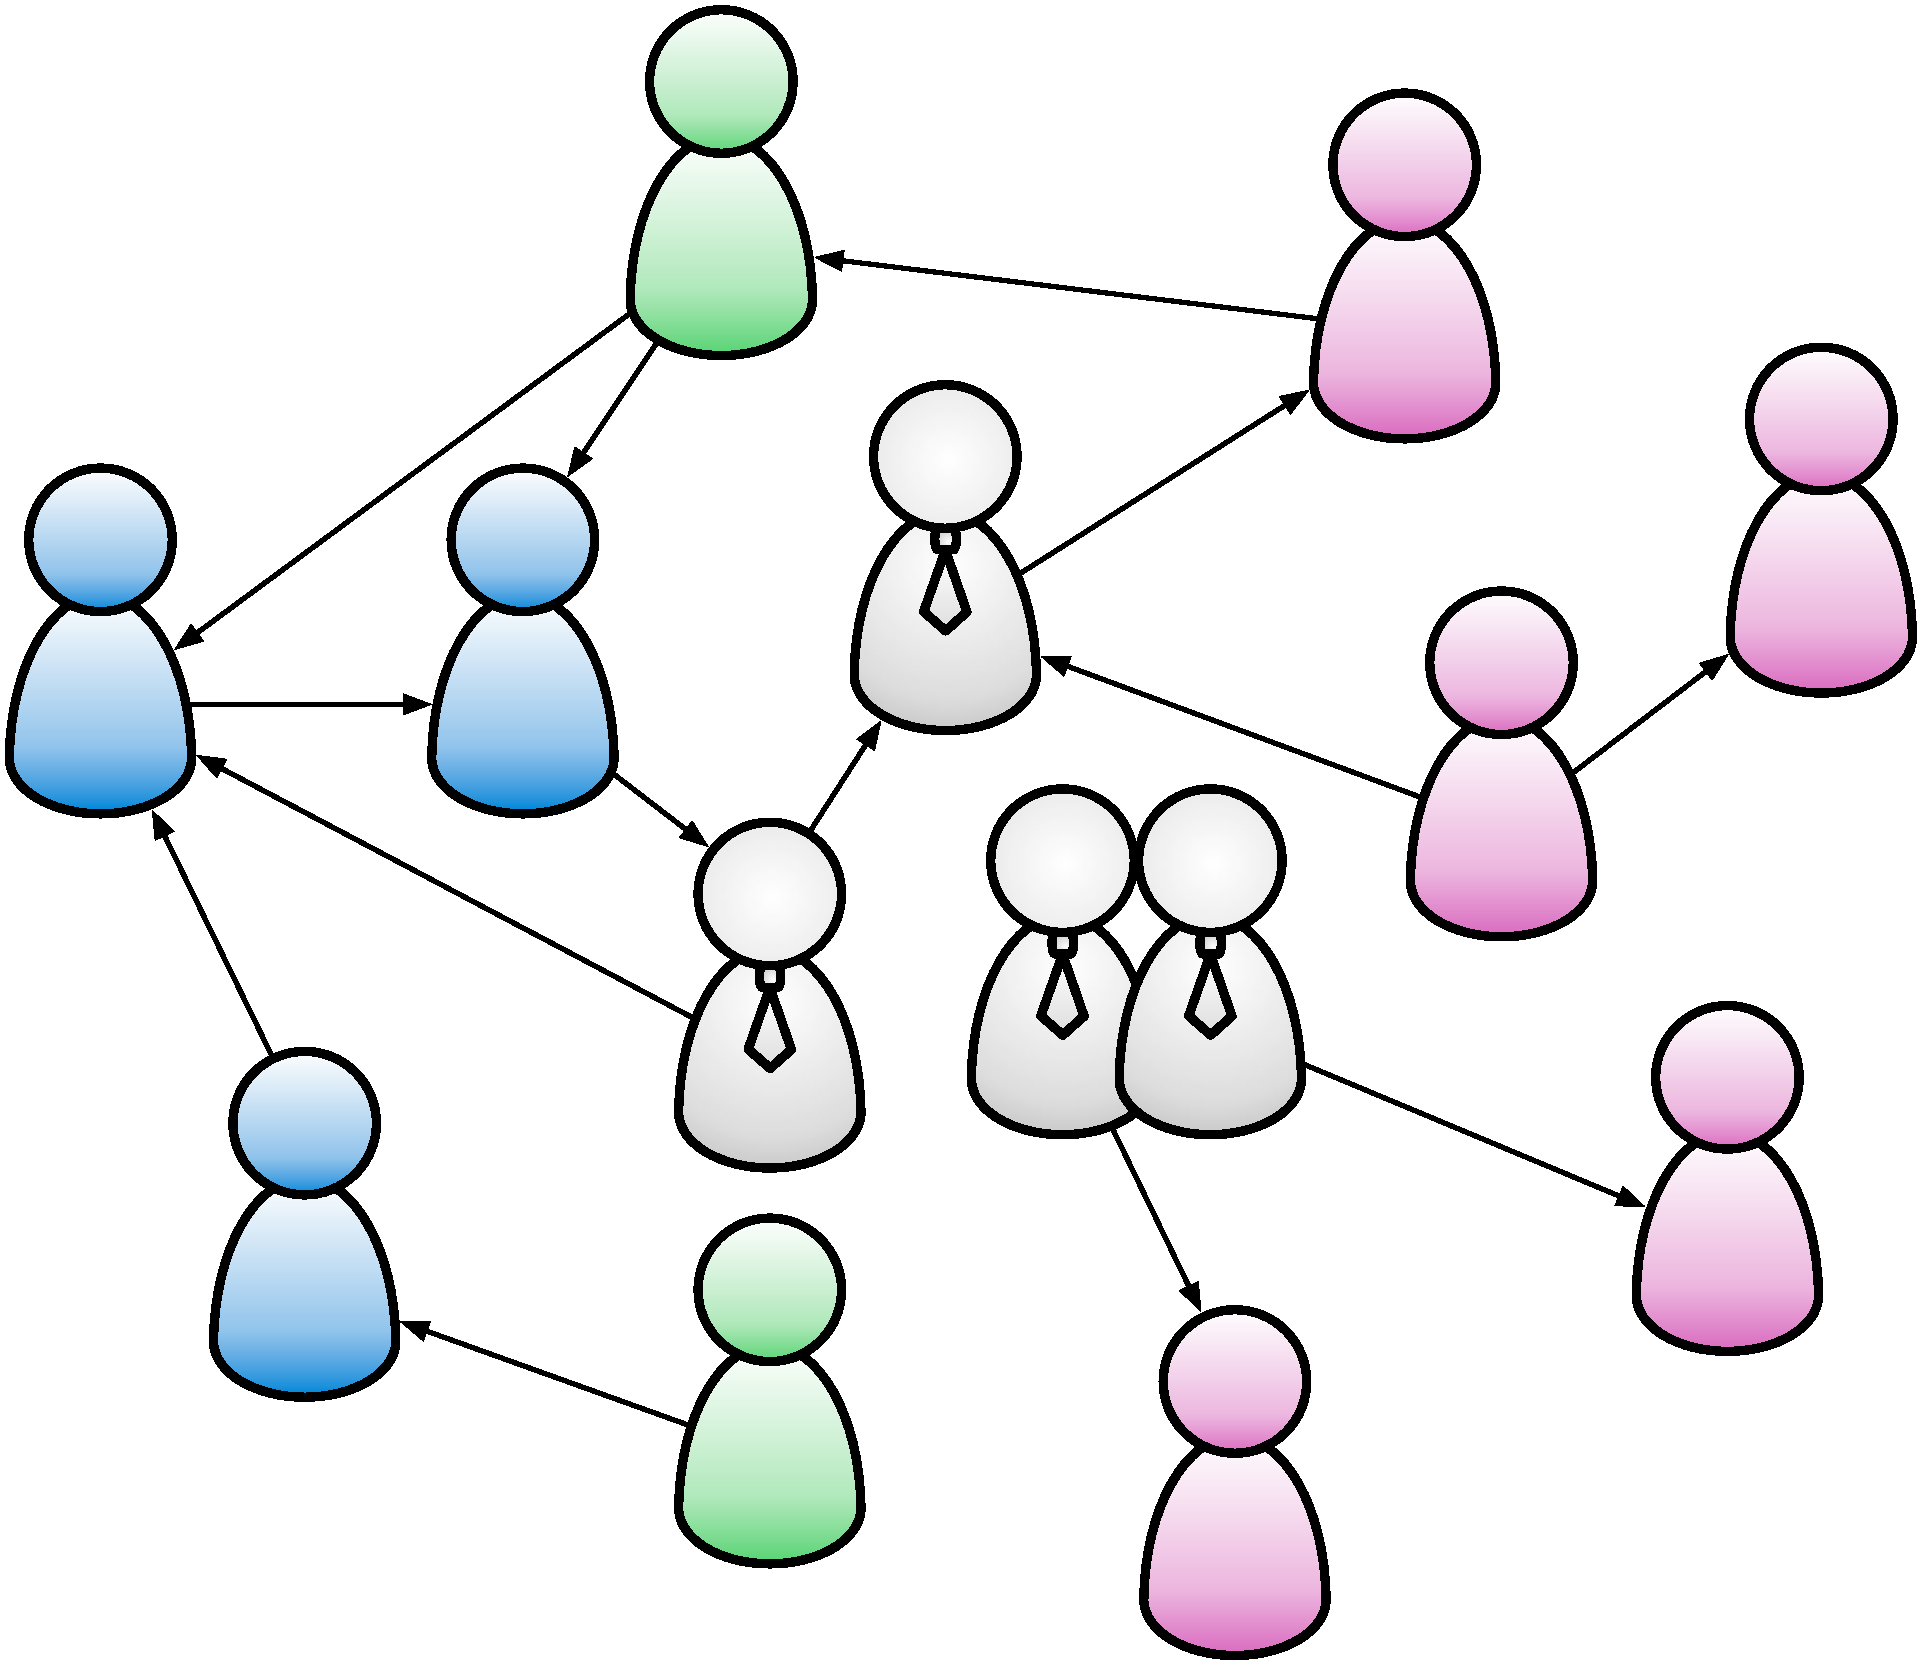
\includegraphics[width=0.40\textwidth,angle=0]{./bilder/analyse/kommunikationswege.pdf}
\caption{Beispiel der unorganisierten Kommunikationswege}
\label{pic:kommunikationswege}
\end{center}
\end{figure}

Das ist auch grundsätzlich nicht zu vermeiden, bzw. das muss zu einem gewissen
Grad auch der Fall sein. Ansonsten wären die Abläufe von wenigen Anlaufstellen abhängig
und das ganze würde ins Stocken geraten. Trotzdem birgt es gewisse Schwachstellen.
Zum Beispiel, dass nicht alle Beteiligten eines Projektes den gleichen Informationsstand 
haben. Dies kann sich beim Kontakt mit einem Kunden negativ auswirken, wenn der
Kunde schon über etwas in Kenntnis gesetzt wurde, und der Mitarbeiter am
Telefon selbst gar noch über die selben Informationen verfügt. Die Schwächen 
werden in der Analyse des Projektablaufes noch genauer beleuchtet.

Der Aufbau einer Beratung, die zur Zeit im Gange ist, soll genau solche Probleme
lösen. Jedoch steckt allink hier noch in den Kinderschuhen und erhofft sich
unteranderem aus dieser Arbeit Erkenntnisse über einen möglichst optimalen 
Projektablauf.
